\documentclass[tikz,dvisvgm]{standalone}
\usetikzlibrary{shapes.geometric, arrows, positioning, fit}

\begin{document}
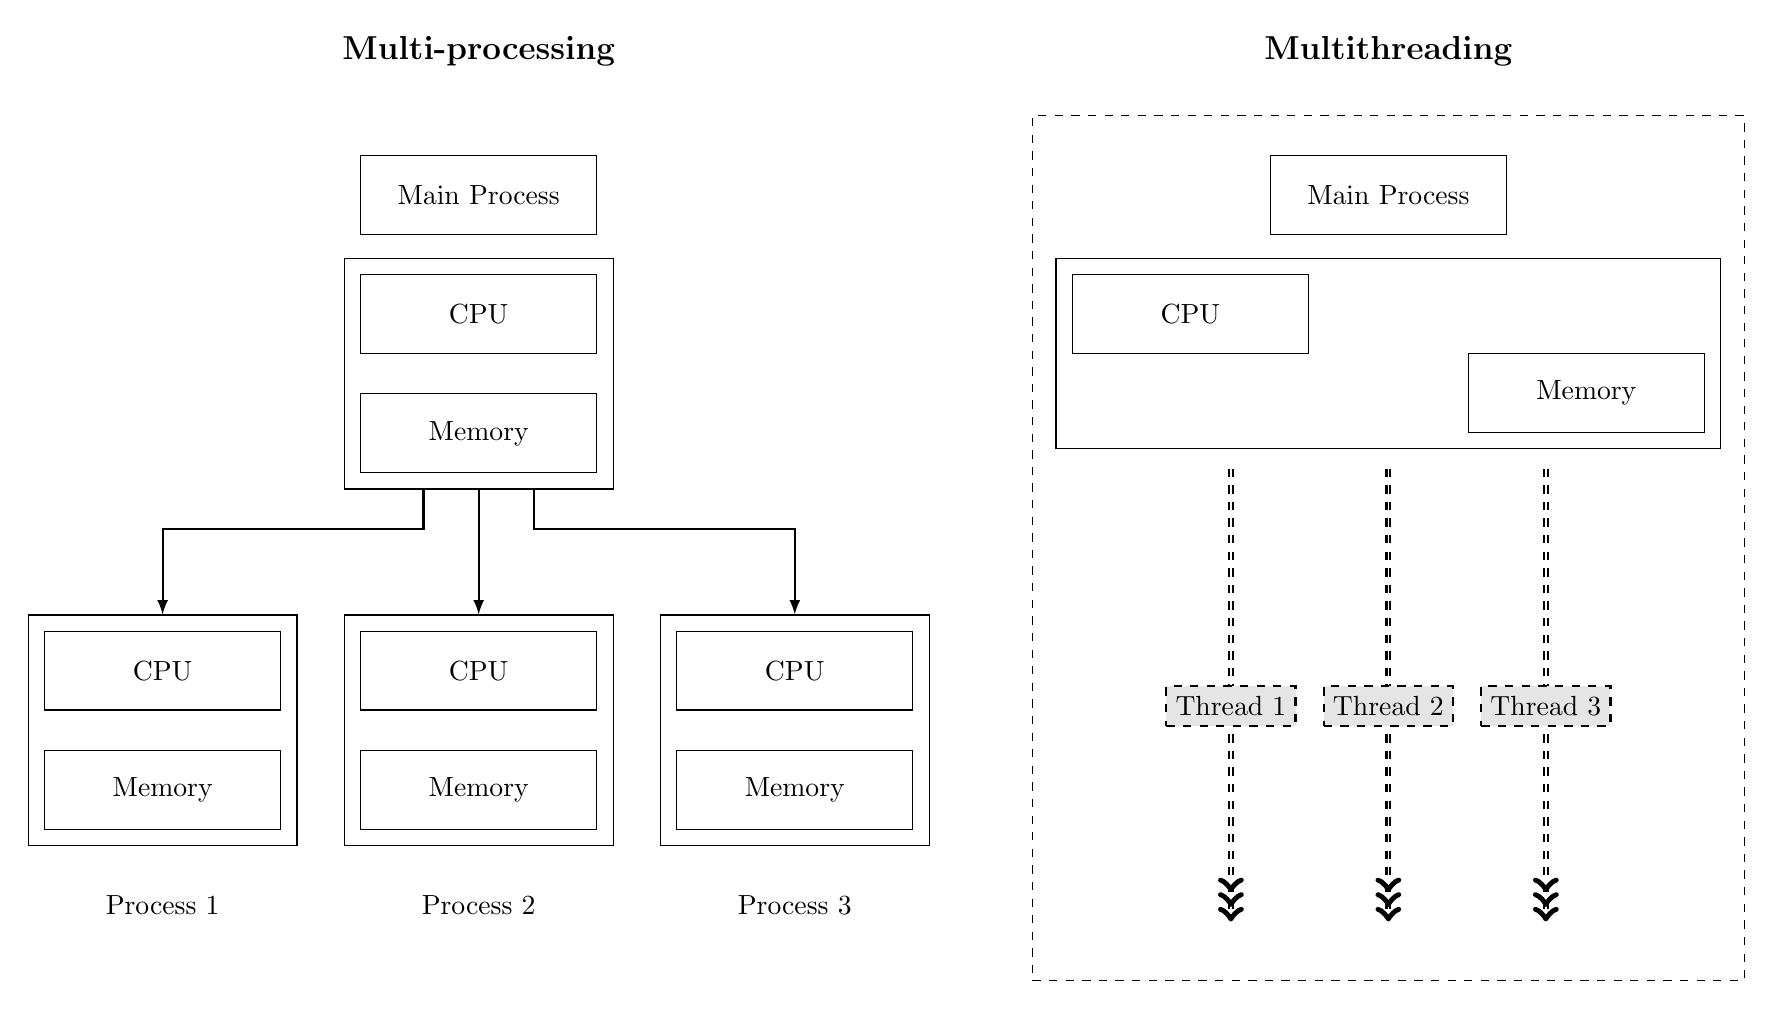
\begin{tikzpicture}[
    process/.style={rectangle, draw, minimum width=3cm, minimum height=1cm},
    thread/.style={rectangle, draw, minimum width=1cm, minimum height=0.5cm, fill=gray!20},
    arrow/.style={-latex, thick},
    dashedarrow/.style={->>>, double,thick, dashed},
    label/.style={font=\large\bfseries}
]

% Label for Multiprocessing
\node[label] (multiprocessing_label) at (0, 0) {Multi-processing};

% Multiprocessing
\node[process, below=1cm of multiprocessing_label] (main1) {Main Process};
\node[process, below=0.5cm of main1] (cpu1) {CPU};
\node[process, below=0.5cm of cpu1] (memory1) {Memory};

% Box around CPU and Memory in Multiprocessing
\node[draw, fit=(cpu1) (memory1), inner sep=0.2cm] (multiprocessing) {};

% Subprocesses
\node[process, below left=2cm and 1cm of memory1] (sub1cpu) {CPU};
\node[process, below=0.5cm of sub1cpu] (sub1mem) {Memory};
\node[draw, fit=(sub1cpu) (sub1mem), inner sep=0.2cm] (sub1box) {};
\node[below=0.5cm of sub1box] (sub1label) {Process 1};

\node[process, below=2cm of memory1] (sub2cpu) {CPU};
\node[process, below=0.5cm of sub2cpu] (sub2mem) {Memory};
\node[draw, fit=(sub2cpu) (sub2mem), inner sep=0.2cm] (sub2box) {};
\node[below=0.5cm of sub2box] (sub2label) {Process 2};

\node[process, below right=2cm and 1cm of memory1] (sub3cpu) {CPU};
\node[process, below=0.5cm of sub3cpu] (sub3mem) {Memory};
\node[draw, fit=(sub3cpu) (sub3mem), inner sep=0.2cm] (sub3box) {};
\node[below=0.5cm of sub3box] (sub3label) {Process 3};

% Connections
\coordinate [left=0.7cm of multiprocessing.south] (subwest);
\draw[arrow] (subwest) -- ++(0,-0.5) -| (sub1box.north);
\draw[arrow] (multiprocessing.south) --  (sub2box.north);
\coordinate [right=0.7cm of multiprocessing.south] (subeast);
\draw[arrow] (subeast) -- ++(0,-0.5) -| (sub3box.north);

% Label for Multithreading
\node[label, right=8cm of multiprocessing_label] (multithreading_label) {Multithreading};

% Multithreading
\node[process, below=1cm of multithreading_label] (main2) {Main Process};
\node[process, below right=1.5cm and -0.5cm of main2] (memory2) {Memory};
\node[process, below left=0.5cm and -0.5cm of main2] (cpu2) {CPU};

% Box around CPU and Memory in Multithreading
\node[draw, fit=(cpu2) (memory2), inner sep=0.2cm] (multithreading_cpu_mem) {};

% Threads
\node[below=0cm of multithreading_cpu_mem, xshift=-2cm] (thread1top) {};
\node[below=0cm of multithreading_cpu_mem] (thread2top) {};
\node[below=0cm of multithreading_cpu_mem, xshift=2cm] (thread3top) {};

\node[below=6cm of multithreading_cpu_mem, xshift=-2cm] (thread1bottom) {};
\node[below=6cm of multithreading_cpu_mem] (thread2bottom) {};
\node[below=6cm of multithreading_cpu_mem, xshift=2cm] (thread3bottom) {};

\draw[dashedarrow] (thread1top) -- (thread1bottom) node[thread, below=3cm of multithreading_cpu_mem,xshift=-2cm] {Thread 1};
\draw[dashedarrow] (thread2top) -- (thread2bottom) node[thread, below=3cm of multithreading_cpu_mem] {Thread 2};
\draw[dashedarrow] (thread3top) -- (thread3bottom) node[thread, below=3cm of multithreading_cpu_mem,xshift=2cm] {Thread 3};


% % Box around the entire multithreading section
\node[draw, dashed, fit=(main2) (cpu2) (memory2) (thread1bottom) (thread2bottom) (thread3bottom), inner sep=0.5cm] (multithreading) {};

\end{tikzpicture}
\end{document}